\documentclass{article}      % Specifies the document class
\usepackage{caption}
\usepackage[final]{graphicx}
\usepackage{amsmath}
\usepackage{placeins}
\title{Case Study 1: Superconductor Dataset - Prediction of Critical Temperature and Interpretation of Superconducting Material Properties}  % Declares the document's title.
\author{Kristin Henderson}   % Declares the author's name.
\date{May 12, 2025}          % Deleting this command produces today's date.

\newcommand{\ip}[2]{(#1, #2)}
                             % Defines \ip{arg1}{arg2} to mean
                             % (arg1, arg2).
                             
\begin{document}             % End of preamble and beginning of text.

\maketitle                   % Produces the title.

\section{Introduction}       % Produces section heading.  Lower-level
                             % sections are begun with similar
                             % \subsection and \subsubsection commands.

This study aims to identify important properties of superconductors, materials that give little or no resistance to electrical current, and to predict the critical temperature at which their superconducting properties operate.

The Superconductivity Dataset is a University of Califonia at Irvine Machine Learning Repository dataset. It contains 21,263 entries consisting of 82 features. The dataset contains two files, one containing material properties, which are numeric features, and the other containing the chemical formula encoded by a vectorized format, with each element represented as a feature and the value being the number of atoms. The target variable is the \emph{superconducting critical temperature} in Kelvin. There is no missing data.

Table 1 contains the material properties, i.e. the category of features, and their descriptions.

\begin{table}[h!]
    \captionof{table}{Category of Features in the Superconductivity Dataset} 
    \centering
    \begin{tabular}{|l|l|}
    \hline
    \textbf{Variable} & \textbf{Description} \\ \hline \hline
    number\_of\_elements & unique elements in the material \\ \hline
    atomic\_mass & atomic mass of the compositional elements \\ \hline
    fie & first ionization energy \\ \hline
    atomic\_radius & atom size \\ \hline
    Density & mass per unit volume \\ \hline
    ElectronAffinity & energy change when electron is added to neutral atom \\ \hline
    FusionHeat & heat required to change solid to liquid \\ \hline
    ThermalConductivity & ability to conduct heat \\ \hline
    Valence & combining capacity of elements \\ \hline
    material & chemical formula \\ \hline
    \end{tabular}
    \label{table:basic_properties}
\end{table}

Table 2 lists the statistical metrics for each property of the materials. Each of the properties (except \texttt{number\_of\_elements} and \texttt{material}) is represented by all ten metrics listed in Table 2, resulting in multiple features per property.

\begin{table}[h!]
    \captionof{table}{Statistical Metrics of Each Material's Property} 
    \centering
    \begin{tabular}{|l|l|}
    \hline
    \textbf{Metric} & \textbf{Description} \\ \hline \hline
    mean & average value \\ \hline
    wtd\_mean & weighted mean \\ \hline
    gmean & geometric mean \\ \hline
    wtd\_gmean & weighted geometric mean \\ \hline
    entropy & distribution of values \\ \hline
    wtd\_entropy & weighted entropy \\ \hline
    range & difference between max and min values \\ \hline
    wtd\_range & weighted range \\ \hline
    std & standard deviation \\ \hline
    wtd\_std & weighted standard deviation \\ \hline
    \end{tabular}
    \label{table:statistical_measures}
\end{table}

A linear regression model is chosen for several reasons. Primarily, it is an appropriate choice with the goal of predicting a continuous variable and having the ability to identify and explain the most important features in determining the critical temperature. Secondarily, a linear model is a good choice for computational efficiency.

The target variable in a linear regression model is a linear combination of the input features.
\[ y = m_0x_0 + m_1x_1 + \cdots + m_nx_n \text{ where } x_0 = 1 \text{ and } m_0 \text{ is the intercept.} \]
Penalized linear regression models with different types of regularization are used as a tool to prevent overfitting. Penalty terms are added to the base loss function:
\[ MSE = \frac{1}{n} \sum_{i=1}^{n} \left(Y_i - \sum_{j=0}^{k} m_j x_{ij}\right)^2 \]
Here I compare LASSO, which uses a first-order L1 penalty term \( \lambda \sum_{j=0}^{k} |m_j| \) to Ridge regression with its second-order L2 penalty term \( \lambda \sum_{j=0}^{k} m_j^2 \). For interpretability of error in the model and to get a sense of its usefulness and practicality, I will also compute the root mean squared error (RMSE) from the chosen loss metric, mean squared error (MSE).

\section{Data}
Many of the features in this dataset are different statistical metrics of the same general property. For example, \texttt{FusionHeat} the heat required to change a solid to a liquid, is represented by 10 features: mean, weighted mean, geometric mean, weighted geometric mean, entropy, weighted entropy, range, weighted range, standard deviation and weighted standard deviation. These likely are necessary to describe the material based on the different atoms in its composition. Generally, the middle fifty percent of all the features are roughly symmetric. Some categories of features have outliers, more high than low, and some are skewed, especially in their outer range. Boxplots of fusion heat (see Figure \ref{fig:fusionheat_boxplots}) and valence (see Figure \ref{fig:valence_boxplots}) are representative of variables with, respectively, smaller and larger ranges, greater and lesser skewness, and more and fewer outliers.

\begin{figure}[h]
	\centering
	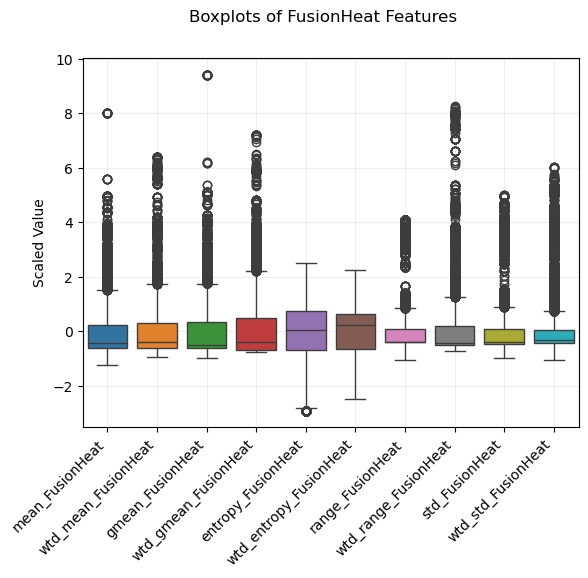
\includegraphics[width=0.85\textwidth]{figures/plt_box_fusionHeat.png}
	\caption{Boxplots of \texttt{FusionHeat} features. Notice relatively small ranges for the middle 50\% of the data, some right skewness, and high outliers. Values were scaled (z-scored) using \texttt{StandardScaler} a function within the scikit-learn package, to compare on the same scale and axis while preserving the distributions.}
	\label{fig:fusionheat_boxplots}
\end{figure}

\begin{figure}[h]
	\centering
	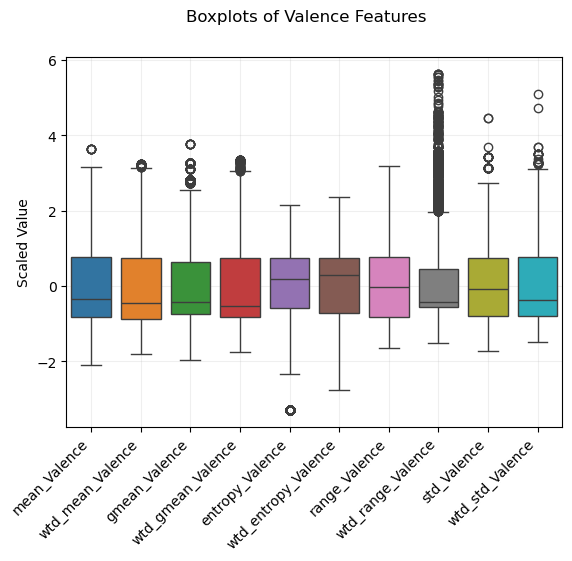
\includegraphics[width=0.85\textwidth]{figures/plt_box_valence.png}
	\caption{Boxplots of \texttt{Valence} features. Notice broader ranges for the middle 50\% of the data and few outliers. Values were scaled (z-scored) using \texttt{StandardScaler} to compare on the same scale and axis while preserving the distributions.}
	\label{fig:valence_boxplots}
\end{figure}

Despite many of the features being different metrics of the same property, no features were perfectly correlated. Without sufficient domain knowledge to determine that some could be excluded, all features were included in the modeling process.

The distribution of the target variable, critical temperature, is right-skewed with a range from 0 to 185 Kelvin, shown in Figure \ref{fig:critTemp_hist}. Over one third of the entries fall within the 0 to 10 Kelvin range. I also plotted a histogram of the log-transformed critical temperature, shown in Figure \ref{fig:critTempLog_hist}, but the transformation did not fully rectify the skewness. I chose to continue the modeling process without log-transforming the target variable to make interpretation of errors and the coefficients more straightforward.

\begin{figure}[h]
	\centering
	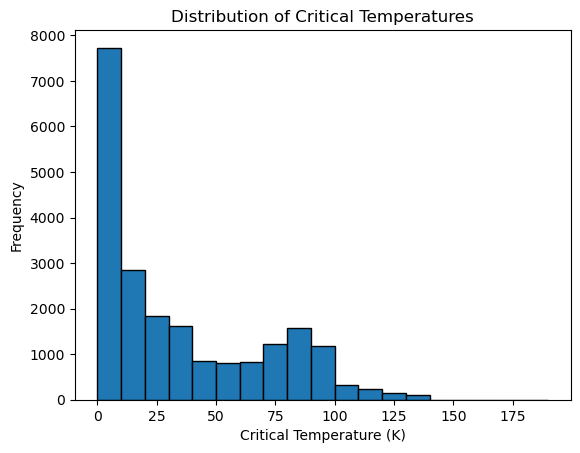
\includegraphics[width=0.85\textwidth]{figures/plt_hist_critTemp.png}
	\caption{Histogram of the target data, critical temperature. Notice that over 35\% of the values fall within the 0-10 K bin.}
	\label{fig:critTemp_hist}
\end{figure}

\begin{figure}[h]
	\centering
	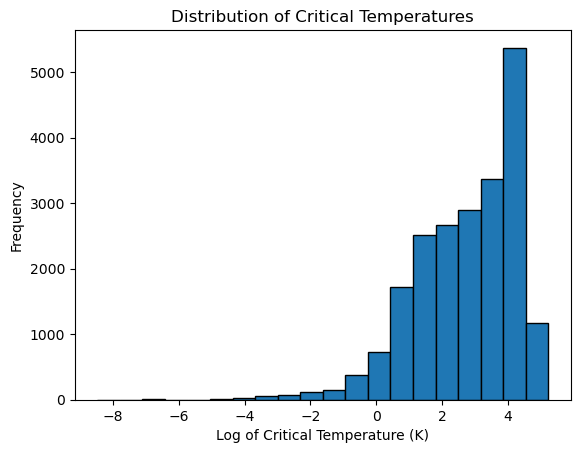
\includegraphics[width=0.85\textwidth]{figures/plt_hist_critTempLog.png}
	\caption{Histogram of the target data, critical temperature after log transformation. Notice that the distribution is not fully normal.}
	\label{fig:critTempLog_hist}
\end{figure}

Though some of the feature have outliers, more commonly high ones, none seem to be unusually abnormal or suggest an error in the data. Given that, and the fairly normal distribution of the data, particularly the reasonable symmetry within the interquartile ranges (IQR), I choose to stick with \texttt{StandardScaler}. I choose to scale only the numerical material property features and not to scale the vector encoded chemical formula features.

\section{Modeling}
Five-fold cross validation with a random shuffling of the data was used for hyperparameter tuning. The out-of-fold predictions were used to calculate the MSE. A manual grid search of the penalty term \(\lambda \) was performed for both LASSO and Ridge models, starting with a broad range of values to identify a region likely to optimize the loss. Using the lowest MSE, the best \(\lambda \) for each model was chosen from a second, narrower search. For LASSO, the \(\lambda \) values searched ranged from 0.5 to 10, focusing on smaller increments under 1, while for Ridge the values ranged from \(10^{-5}\) to \(10^{4}\) increasing by orders of magnitude with finer increments toward the upper end of that range.
I also chose to tune an ElasticNet model as a comparison to the pure L1 or L2 regularization of the LASSO or Ridge models respectively. For ElasticNet a grid search was conducted for both the penalty term, \(\lambda \), with values in the range from  \(10^{-3}\) to \(10^{3}\), and for the L1 mixing term from 0.01 to 0.9, focusing for both hyperparameters particularly on the values between 0.01 and 0.1.

\section{Results}

Tuning curves for the LASSO and Ridge models are shown in Figure \ref{fig:tuning_L1} and Figure \ref{fig:tuning_L2}, respectively. The estimated MSE on out-of-fold predictions for LASSO with an optimized \(\lambda \) of 0.34 was \( 332.03 \pm 16.00 \) (mean \(\pm\) standard deviation) and for Ridge regression with an optimized \(\lambda \) of 2000 was \( 333.28 \pm 25.46 \). 

\begin{figure}[h]
	\centering
	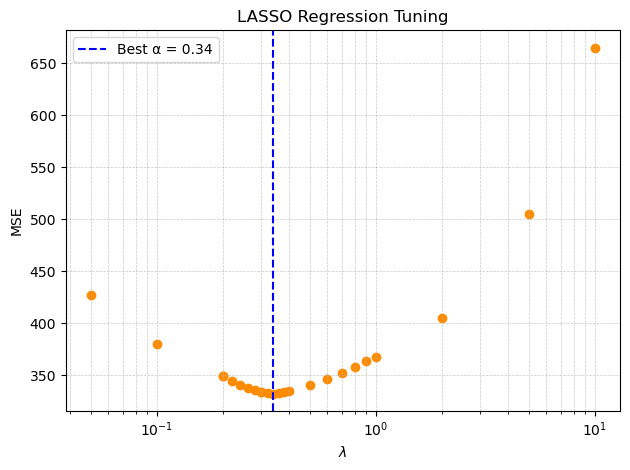
\includegraphics[width=0.85\textwidth]{figures/plt_tuning_L1.png}
	\caption{Tuning Curve of  \(\lambda \) for the LASSO model. The optimum value of \(\lambda \) is indicated by the dotted blue line.}
	\label{fig:tuning_L1}
\end{figure}

\begin{figure}[h]
	\centering
	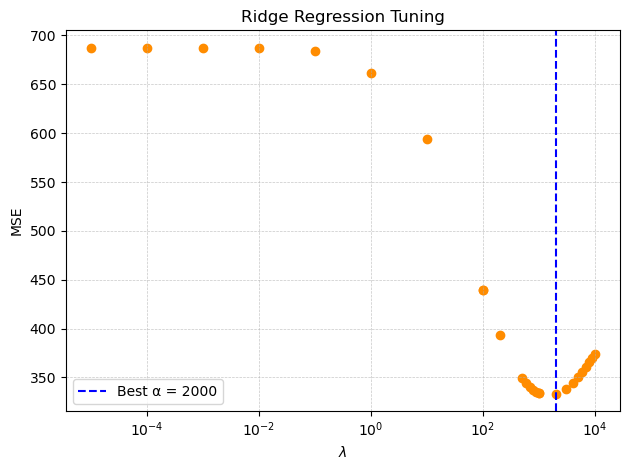
\includegraphics[width=0.85\textwidth]{figures/plt_tuning_L2.png}
	\caption{Tuning Curve of  \(\lambda \) for the Ridge regression model. Again, the optimum value of \(\lambda \) is indicated by the dotted blue line.}
	\label{fig:tuning_L2}
\end{figure}

The results of a narrowed range of the ElasticNet grid search can be seen in Figure \ref{fig:tuning_EN}. The estimated MSE on out-of-fold predictions for ElasticNet with an optimized \(\lambda \) of 0.1 and mixing term of 0.09 was \( 332.27 \pm 30.31 \). For comparison to all the regularized models, a ordinary least squares regression model yielded an MSE of \(  687.55 \pm 584.20 \).

A plot of residuals versus the observed critical temperature values for both the LASSO and Ridge models display a slight upward trend and fan shape with a few extreme points, shown in Figure \ref{fig:residL1} and Figure \ref{fig:residL2}.

\begin{figure}[h]
	\centering
	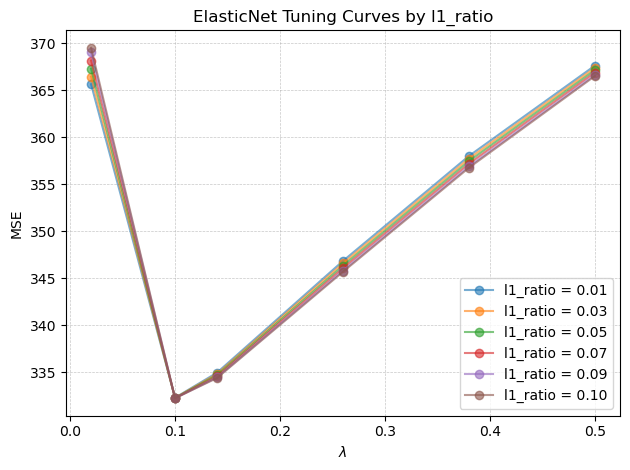
\includegraphics[width=0.85\textwidth]{figures/plt_tuning_EN_narrowLine.png}
	\caption{Tuning Curve of  \(\lambda \) using different mixing terms for the ElasticNet regression model.}
	\label{fig:tuning_EN}
\end{figure}

\begin{figure}[h]
        \centering
        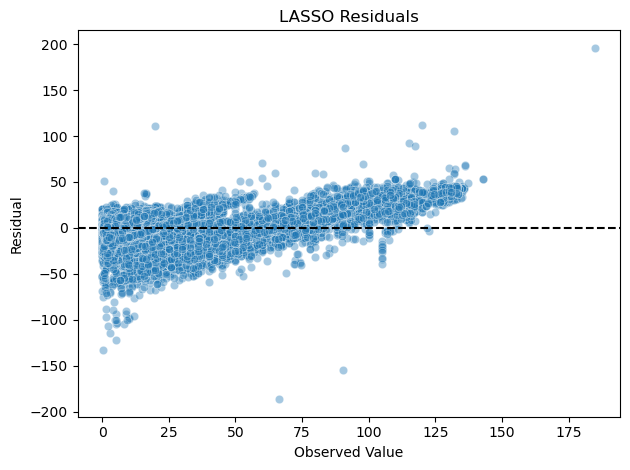
\includegraphics[width=0.85\textwidth]{figures/plt_residuals_L1.png}
        \caption{Residuals of the predictions plotted versus the observed values for the LASSO model show a slight upward trend and fan shape and a few extreme values.}
\label{fig:residL1}
\end{figure}

\begin{figure}[h]
        \centering
        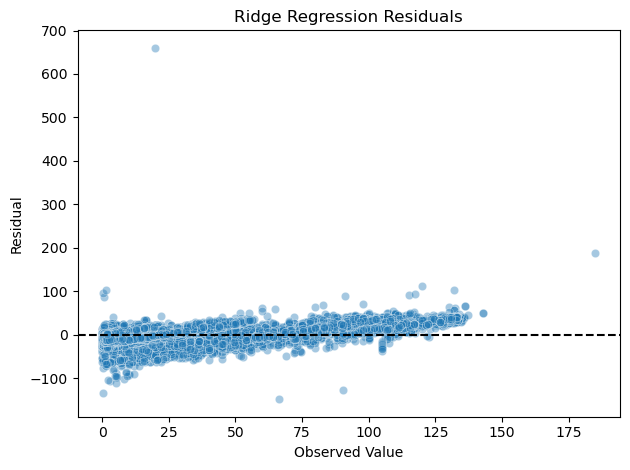
\includegraphics[width=0.85\textwidth]{figures/plt_residuals_L2.png}
        \caption{Residuals of the predictions ploted versus the observed values show a slight upward trend and fan shape and a few extreme values.}
\label{fig:residL2}
\end{figure}

The most important properties and chemical components of superconductors identified by the LASSO model, which achieved the lowest MSE and smallest standard deviation, are listed in Table~\ref{table:lasso_coefficients} along with their coefficients, indicators of the importance and direction of their relationship with the target variable. Interestingly, the most important elements in the chemical makeup are Barium, Bismuth, and Calcium. Unsurprisingly, several of the metrics of thermal conductivity are important in predicting the conductive temperature of a material. The range of the atomic mass, and metrics of valence and electron affinity are also important features.

\FloatBarrier
Table 3 contains the 10 most important features and their coefficients from the LASSO model.

\begin{table}[h!]
    \centering
    \captionof{table}{Most Important Features from the LASSO Model} 
    \begin{tabular}{|l|l|}
    \hline
    \textbf{Variable} & \textbf{Coefficient} \\ \hline \hline
    Ba & 9.66 \\ \hline
    wtd\_mean\_ThermalConductivity & 9.36 \\ \hline
    wtd\_gmean\_ThermalConductivity & -7.82 \\ \hline
    range\_atomic\_mass & 5.69 \\ \hline
    Bi & 4.70 \\ \hline
    wtd\_std\_Valence & -4.14 \\ \hline
    wtd\_std\_ThermalConductivity & 3.52 \\ \hline
    wtd\_gmean\_ElectronAffinity & -3.49 \\ \hline
    Ca & 3.44 \\ \hline
    wtd\_entropy\_ElectronAffinity & -3.09 \\ \hline
    \end{tabular}
    \label{table:lasso_coefficients}
\end{table}

The most important properties and chemical components of superconductors found using the Ridge regression model are listed in Table~\ref{table:ridge_coefficients} along with their coefficients. These ten features are the same as the top ten features from the LASSO model. Additionally, the signs of the relationship with the target variable, positive or negative are all also the same between the models. However, the variables rank slightly differently, and the coefficients are generally smaller in the Ridge model.

Table 4 contains the 10 most important features and their coefficients from the Ridge regression model.

\begin{table}[h!]
    \centering
    \captionof{table}{Most Important Features from the Ridge Regression Model} 
    \begin{tabular}{|l|l|}
    \hline
    \textbf{Variable} & \textbf{Coefficient} \\ \hline \hline
    Ba & 8.00 \\ \hline
    wtd\_mean\_ThermalConductivity & 4.64 \\ \hline
    wtd\_std\_Valence & -4.57 \\ \hline
    wtd\_std\_ThermalConductivity & 4.09 \\ \hline
    Bi & 4.00 \\ \hline
    wtd\_gmean\_ThermalConductivity & -3.68 \\ \hline
    range\_atomic\_mass & 3.63 \\ \hline
    wtd\_entropy\_ElectronAffinity & -3.32 \\ \hline
    Ca & 3.23 \\ \hline
    wtd\_gmean\_ElectronAffinity & -2.98 \\ \hline
    \end{tabular}
    \label{table:ridge_coefficients}
\end{table}

\section{Conclusion}

All three models which used regularization, Lasso, Ridge, and ElasticNet, achieved statistically equivalent results with similar cross-validated MSEs and overlapping standard deviations. There was little difference in computational efficiency with the exception of ElasticNet, which required tuning an additional parameter. Additionally, the optimum L1 ratio for ElasticNet was 0.09, meaning it is primarily using L1 rather than an balanced combination of L1 and L2 penalties. The LASSO model has a very slightly lower MSE and standard deviation than the others. The RMSEs of each regularization model, reflecting error in the original units, were all 18 Kelvin. In contrast, the unregularized linear regression model had a much higher error, an RMSE of 26 K, and larger variability than the other models.

The trend and fan shape in the residual plots indicate potential heteroscedasticity in the errors. Although the log transformation did not eliminate the skewness in the target variable distribution, it may be worth revisiting the modeling process using the log-transformed variable to try to improve the variance in the residuals and better meet the assumptions of the model.

The LASSO and Ridge models were consistent in their variable importance, with Barium and weighted mean of thermal conductivity being the most important features in determining the critical temperature.

\end{document}
